
\chapter{系统总体设计}
\label{chap:design}

前面两章介绍了本系统的研究目的,要解决的问题和对于这些问题本系统提出的解决方案。虽然第二章中只简单提到了解决方案,而并没有涉及系统具体的逻辑结构。但是从第二章的介绍,也不难看出本文介绍的系统大概的系统架构与主要的功能设置。接下来的两章我们将深入的介绍该系统的逻辑结构和部分实现细节。本章首先介绍系统总的逻辑结构,然后简单介绍一下本系统涉及的技术和开源组件。下一章将通过“文档撰写与展示”、“用户空间逻辑结构”、“社交网络与门户”几个部分,逐步介绍本系统的逻辑结构,并重点介绍\smarkdown语法与RESTful api部分的实现细节。

\section{系统逻辑结构和统一接口}
\label{sec:restful}

前文提到,本系统要实现的一个重要功能就是使用户文档可以方便的在不同种类的设备间传递,这些设备包括运行windows操作系统的PC机、运行mac操作系统的apple机、运行ios平台和android平台手机和平板电脑、运行linux操作系统的实验用机和各种移动阅读设备(电纸书)等等。显然,要实现这样的功能,就要求任何设备上的客户端程序都可以访问系统服务器上的数据,并且访问的方式要相对统一。这样才能尽可能的降低服务器端程序的复杂度,使系统结构尽量紧凑。

面向统一接口的web service服务架构,显然是实现如上功能的不二选择。web service的主要特点就是:平台的兼容性,任何平台的任何客户端只要支持规定的传输格式,都可以便捷的访问服务数据。

web service的常用的方法有:
\begin{enumerate}
\item RPC 所谓的远程过程调用 (面向方法):像调用本地服务(方法)一样调用服务器的服务(方法),通常的实现有XML-RPC,JSON-RPC,通信方式基本相同, 所不同的只是传输数据的格式。
\item SOA 所谓的面向服务的架构(面向消息):前几年炒的很火的一个词, SOA是基于消息的,通常与具体的实现语言无关, 所以在一定程度上得到大公司的支持。
\item REST 所谓的 Representational state transfer (面向资源):是以资源为中心, 名词即资源的地址, 动词即施加于名词上的一些有限操作, 表达是对各种资源形态的抽象。
\end{enumerate}
本系统选择架构比较清晰,可扩展性较好,也是目前被广泛提倡使用的REST结构。REST 是英文 Representational State Transfer 的缩写,是近年来迅速兴起的,一种基于 HTTP,URI,以及 XML 这些现有协议与标准的,针对网络应用的设计和开发方式。它可以降低开发的复杂度,提高系统的可伸缩性。REST 的核心是可编辑的资源及其集合,用符合 Atom 文档标准的 Feed 和 Entry 表示。每个资源或者集合有一个惟一的 URI。系统以资源为中心,构建并提供一系列的 Web 服务。REST 的基本概念和原则包括:系统上的所有事物都被抽象为资源、每个资源对应唯一的资源标识、对资源的操作不会改变资源标识本身、所有的操作都是无状态的等等。

在 REST 中,开发人员显式地使用 HTTP 方法,对系统资源进行创建、读取、更新和删除的操作:
\begin{enumerate}
\item 使用 POST 方法在服务器上创建资源
\item 使用 GET 方法从服务器检索某个资源或者资源集合
\item 使用 PUT 方法对服务器的现有资源进行更新
\item 使用 DELETE 方法删除服务器的某个资源
\end{enumerate}

图~\ref{fig:xfig9}所示为本系统基本的结构图。从图中我们可以看到的基本信息有:
\begin{enumerate}
\item 本系统是以B/ S为基本架构的。
\item 本系统提供基本的WEB用户界面供用户使用,用户可以在任何有浏览器的环境中访问系统,撰写和获取自己的文档资源。
\item 除了以WEB为主的浏览方式以外,系统还提供了标准的Restful的API接口,通过该接口系统可以直接为各种操作系统,甚至移动设备中的本地程序(APP)提供数据。也就是说,用户不仅可以通过浏览器访问本系统,也可以通过安装本地客户端程序访问系统。
\end{enumerate}
通过以上几点,我们不难发现,由于本系统架构设计上的合理。使本系统天生具有很高的开放性。开放Restful的API接口的好处不仅是为用户访问系统提供了方便,更深层次的意义在于。任何组织和个人都可以利用统一接口来编写程序访问本系统中的数据\footnote{当然,这需要一定的授权}。这也就意味着,不管是学校还是第三放组织,在制作其他系统是需要用到教师和学生的文档数据时,就不需要再重新收集和存储,可以通过和本系统的无缝集成来直接获取这些数据。这给老师和学生带来的方便也是不言而喻的,他们起码不用把自己的数据在办理不同业务时重复的整理和提交。只要把这些数据存放到本系统中就可以了。同时我们的数据也不再是信息孤岛,他们可以被搜素引擎检索到\footnote{当然,这是在用户愿意公开的前提下},并通过文档自身的价值引起更多人的关注。

顺便提一下,其实当今,Restful的API接口的应用已经非常流行,大到 google,yahoo等大公司在自己的系统是使用这样的服务,小到刚刚起步的国内的一些小的互联网公司也在做这方面的探索。所以我个人认为,封闭的,自称体系的信息管理系统(erp)的时代已经过去了,取而代之的是以统一接口为驱动的。开放性的网络服务系统。通过开放的接口,和完善的授权机制,我们可以建立更加开放,更加安全,也更加实用的系统。关于统一接口的话题我们就先进行到这里,在系统实现的章节里我们将详细描述本系统的Restful API接口。
\begin{figure}[H]
  \centering
  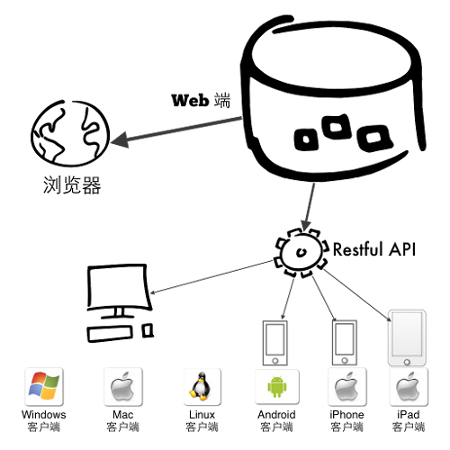
\includegraphics{restful}
  \caption{系统提供web端和restful api接口结构图}
  \label{fig:xfig9}
\end{figure}
通过以上介绍,我们看到,通过系统的统一接口设计从根本上解决了高校用户个人文档管理中不同设备间存取难和不同步的问题,同时也解决了用户在不同场合需要文档数据时,重复整理、重复提交的问题。但是有的时候用户的文档并不满足于自己存取和管理,有的时候我们的用户希望自己的文档可以分发给别人,甚至请别人修改自己的文档。或者和其他人一起合作完成文档。这就需要系统提供一定的社交功能和协作功能。我们将在下面的章节详细讲述本系统社交性和写作性的设计。

\section{系统涉及的实现技术}
\label{sec:language}

本系统要实现的功能繁多,而且要运行的平台也多样\footnote{windows应用,ios app,andriod app,web应用等}。最粗略的统计,主要包括:web service服务端、数据库、web前端、windows客户端和移动客户端几个部分。下面分别进行介绍:

\subsection{web service服务端}
\label{sec:webservice}

上文介绍过,本系统基本架构为restful的web服务。目前支持restful的编程语言和成型的开源架构很多,比如ROR、Python、java、.net等等。本系统选择的后端开发框架为Ruby on Rails,官方简称Rails\cite{ruby2009agile,hartl2012ruby},非正式叫法:RoR。它是使用Ruby\cite{thomas2004programming}脚本语言\footnote{一种为简单快捷面向对象编程而创的脚本语言,在20世纪90年代由日本人松本行弘开发。}所开发的Web开发框架。Rails是一套专业的开发框架,采用了MVC(Model-View-Control)模式、原生支持单元测试和整体测试、支持Ajax和RESTful结构、ORM机制,以及支持各种最新的业界标准像是HTML5、JQuery等等功能。它的发明人是David Heinemeier Hanson(DHH),DHH是2004年将Rails从37signals商业产品中独立出来的开源项目。它的设计目标是只要开发者熟悉它的惯例,就可以快速的开发网站。相比其他的语言和框架,Rails可以让你用更少的编码实现更多的功能。

选择Ruby on Rails的重要原因是:
\begin{itemize}
\item 它对RESTful的支持较好。可以说是原生支持,不用做任何配置就可以构建RESTful的web。
\item 支持多种格式的信息返回,一个后台服务可以支持web段程序,也可以提供api给其他客户端程序使用。
\item 采用它后生产力的暴增,写的的应用程序,增加新的功能都很容易。可以用更少的程序做更多的事情,而且程序维护起来更加容易。
\end{itemize}

当然Rails只是后台服务的基础架构,要完成本系统的诸多负载功能,还需要利用许多开源组件。

\subsection{数据库}
\label{sec:database}

本系统在数据库的使用上与传统的信息管理系统不同,本人将使用传统关系型数据库和非关系型数据库(nosql)相结合的方法。关系型数据库本人将使用开源的数据库mysql\cite{dubois2003mysql}。关于这个数据库这里不过多的介绍,它是目前业界最常使用的开源关系型数据库系统。关于nosql,下面简单的做一个介绍。

nosql的主要特点包括非关系型、分布式、开源、水平可扩展。第一次看到这个名字,很多人都会认为nosql\cite{tiwari2011professional,strauch2011nosql,membrey2010definitive}是“no sql”的简写,所以认为它是sql数据库的替代品,但实际上它是“not only sql”的简写,意思是不止用sql。它的出现主要是弥补关系型数据库的诸多缺点和不足:
\begin{enumerate}
\item 不擅长处理大量数据并发写入的应用。这也是近年来对关系型数据库的最大的诟病,因为通过增加硬件规模和性能来提高数据库读性能,但是由于数据一致性问题想提高写入性能会非常麻烦。进入web2.0时代,关系型数据库应对大量的SNS类型的动态网站时已经显得力不从心。
\item 不擅长处理字段不固定的应用。如果字段不固定,使用关系型数据库非常麻烦,尤其是目前主流的开发框架都使用数据库映射功能(ORM),如果字段不固定,那么开发的难度将非常大。
\end{enumerate}
而nosql数据库则可以很好的解决以上的问题:
\begin{enumerate}
\item nosql易于数据分散,可以通过简单的横向扩展来提高系统性能,而且读写性能均可以通过增加硬件规模和性能来得到线性的提升。
\item nosql可以轻松应对字段不固定的应用。
\end{enumerate}
通过第三章的介绍,本人知道,本人的系统既是一个高并发写入的SNS类的应用,同时也是一个字段不固定的应用。所以同时使用关系型数据库和nosql将很好的解决系统数据存储的问题。


目前常用的nosql数据库大致分为四种:
\begin{enumerate}
\item Key-value stores键值存储, memcached、Tokyo Tyrant、Redis等数据库属于这种类型。
\item Table-oriented 面向表, 主要代表有Google的BigTable和Cassandra。
\item Document-oriented面向文档,最常用的MongoDB 和 CouchDB。
\item Graph-oriented 面向图论, 如Neo4J。
\end{enumerate}
本系统主要是用的是MongoDB\cite{banker2011mongodb,chodorow2010mongodb,wei2011using}这个面向文档的数据库。一方面,它是目前业界最广泛使用的nosql数据库。另外一方面,它面向文档的数据结构可以不用固定表结构,也支持复杂的查询条件,比较吻合本系统的需求。

\subsection{WEB前端}
\label{sec:webui}

对于最终用户,直接面对系统的就是用户界面(UI)。所以系统UI的好坏直接影响系统用户体验。本系统最先实现的也是最主要的用户界面就是WEB端的用户界面,也就是网页版的UI。虽然这么说并不准确,因为现在的WEB已经和几年前的网页大不相同了。WEB技术在近今年发展迅速,从一开始HTML的静态页面和applet小程序,到后来AJAX的流行,再到后来使用FLASH技术的富户端,甚至近两年炒的火热的HTML5。WEB技术的发展速度之快,让所有的WEB开发者叫苦不断,因为永远要学习新的技术。

本系统要使用的WEB前端框架叫做BootStrap,它是2011年twitter\footnote{最早也是世界上最流行的微博系统,被中国网墙屏蔽。}的“一小撮”工程师为了提高他们内部的分析和管理能力,用业余时间为他们的产品构建了一套易用、优雅、灵活、可扩展的前端工具集。Bootstrap由MARK OTTO和Jacob Thornton所设计和建立,在github上开源之后,迅速成为该站上最多人watch和fork的项目。大量工程师踊跃为该项目贡献代码,社区惊人地活跃,代码版本进化非常快速,官方文档质量极其高(可以说是优雅),同时涌现了许多基于Bootstrap建设的网站:界面清新、简洁;要素排版利落大方,如图~\ref{fig:xfig14}所示。

其次,系统门户界面可以使用Jekyll的模板系统,用户可以选择自己门户界面的模板。有兴趣的用户甚至可以自己编写门户模板提供给系统使用。

\begin{figure}[H]
  \centering
  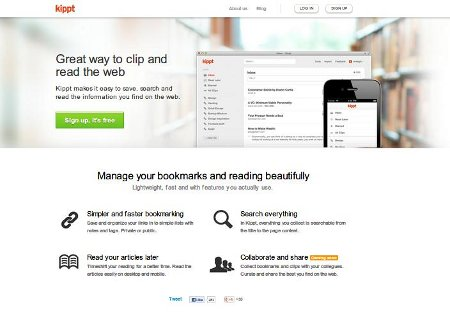
\includegraphics{bootstrap}
  \caption{Bootstrap界面}
  \label{fig:xfig14}
\end{figure}

\subsection{pc客户端和移动客户端}
\label{sec:pcandriodmac}

各种本地客户端程序可以通过标准的RESTful api访问系统数据。任何组织和个人在经过许可的情况下都可以开发并发布本系统的客户端程序。除此以外,本人也会提供官方的客户端程序。根据用户操作习惯的不同那个可以选择WEB方式或者本地客户端形式访问系统。下面简单介绍一下各种本地程序所使用的技术:
\begin{description}
\item[windows客户端] 主要采用c\#语言配合客户端界面的控件实现。
\item[Linux客户端] 使用C++和qt用户界面库实现。
\item[Mac客户端] 使用object c和cocoa开发框架实现。
\item[andriod客户端] 使用java和android开发套件实现。
\item[IOS客户端] 使用object c和Cocoa Touch框架实现。
\end{description}

除以上介绍的语言与框架外,任何编程语言与开发框架都可以用来开发本系统的本地客户端程序。

本章我们简单介绍了本系统的基本的逻辑结构和设计的实现技术,对于系统的各大模块的设计和实现还没有介绍。下一章我们将进入实际的系统设计与实现过程,将更多的讲解本章没有设计到的功能模块的设计,和一部分实现细节。